
\section{Vector Fields}
\label{sec-1}
\label{sec:vector}

Many objects in our natural environment exhibit directional
features that are naturally represented by vector data. Vector
fields, commonly found in science and engineering, describe the
spatial distribution of a vector variable such as fluid flow or
electromagnetic forces. A suitable visualization method has to
display both the magnitude and the direction of the vectors at any
point.

This section illustrates two visualization techniques, arrow plots and
stream lines, with the help of the wind direction and speed forecast
published by MeteoGalicia (see Section \ref{sec:animationST} for
details).

\index{Packages!rasterVis@\texttt{rasterVis}}
\index{Packages!raster@\texttt{raster}}
\index{Data!Wind Speed}

\lstset{language=R,numbers=none}
\begin{lstlisting}
library(raster)
library(rasterVis)

wDir <- raster('data/wDir')/180*pi
wSpeed <- raster('data/wSpeed')
windField <- stack(wSpeed, wDir)
names(windField) <- c('magnitude', 'direction')
\end{lstlisting}

\subsection{Arrow Plot}
\label{sec-1-1}
A frequent vector visualization technique is the arrow plot, which
draws a small arrow at discrete points within the vector field
(Figure \ref{fig:vectorplot}). This approach is best suited for
small datasets. If the grid of discrete points gets too dense or
if the variations in magnitude are too big, the images tend to be
visually confusing.

\index{vectorplot@\texttt{vectorplot}}
\lstset{language=R,numbers=none}
\begin{lstlisting}
vectorplot(windField, isField=TRUE, par.settings=BTCTheme(),
	   colorkey=FALSE, scales=list(draw=FALSE))
\end{lstlisting}

\begin{figure}[htb]
\centering
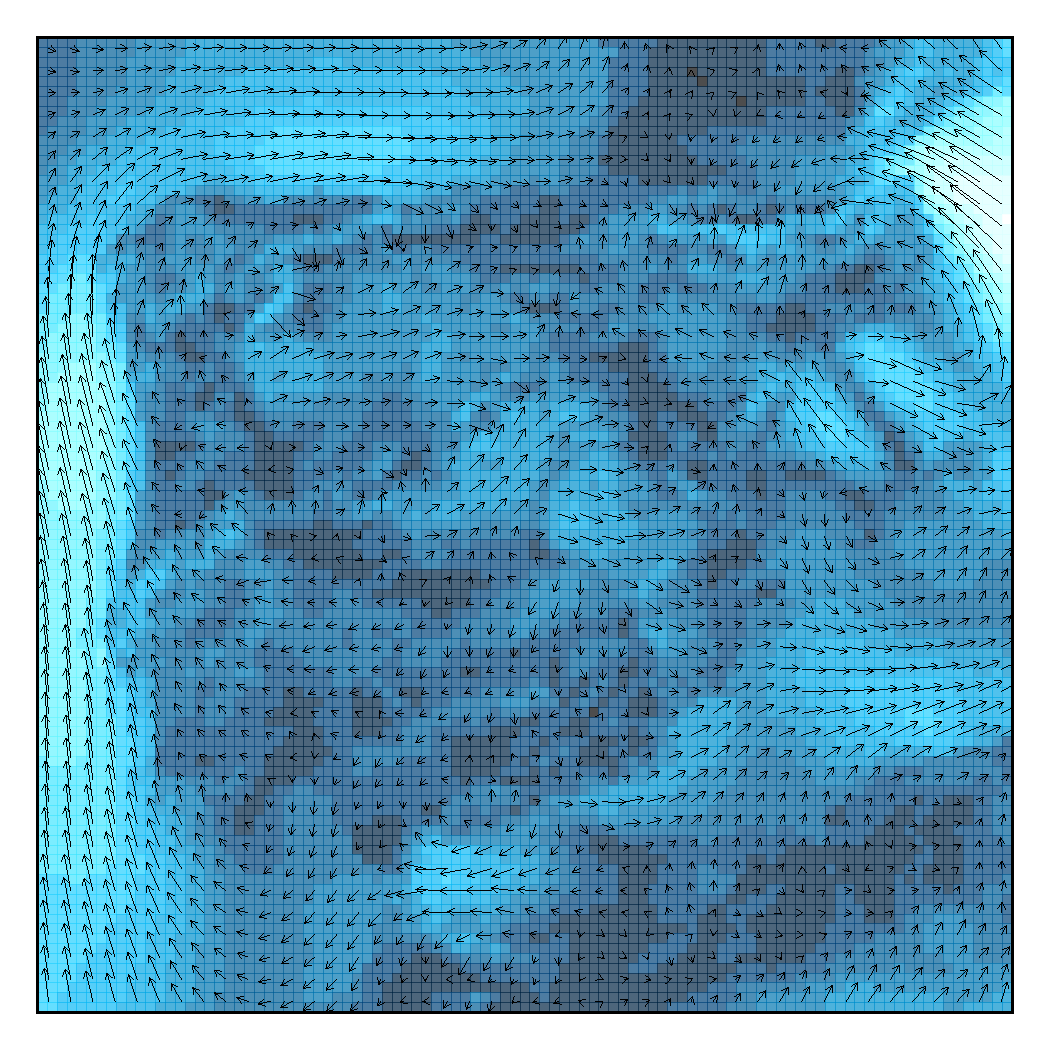
\includegraphics[width=.9\linewidth]{figs/vectorplot.pdf}
\caption{\label{fig:vectorplot}Arrow plot of the wind vector field.}
\end{figure}
\subsection{Streamlines}
\label{sec-1-2}
Another solution is to depict the directional structure of the vector
field by its integral curves, also denoted as flow lines or
streamlines. There are a variety of algorithms to produce such
visualization. The \texttt{streamplot} function of \texttt{rasterVis} displays
streamlines with a procedure inspired by the FROLIC algorithm: For
each point, \emph{droplet}, of a jittered regular grid, a short streamline
portion, \emph{streamlet}, is calculated by integrating the underlying
vector field at that point. The main color of each streamlet indicates
local vector magnitude. Streamlets are composed of points whose sizes,
positions, and color degradation encode the local vector direction
(Figure \ref{fig:streamplot}).

\index{streamplot@\texttt{streamplot}}
\index{brewer.pal@\texttt{brewer.pal}}
\lstset{language=R,numbers=none}
\begin{lstlisting}
myTheme <- streamTheme(region=rev(brewer.pal(n=4, name='Greys')),
				    symbol=BTC(n=9, beg=20))
streamplot(windField, isField=TRUE,
	   par.settings=myTheme,
	   droplet=list(pc=12),
	   streamlet=list(L=5, h=5),
	   scales=list(draw=FALSE),
	   panel=panel.levelplot.raster)
\end{lstlisting}

\begin{figure}[htb]
\centering
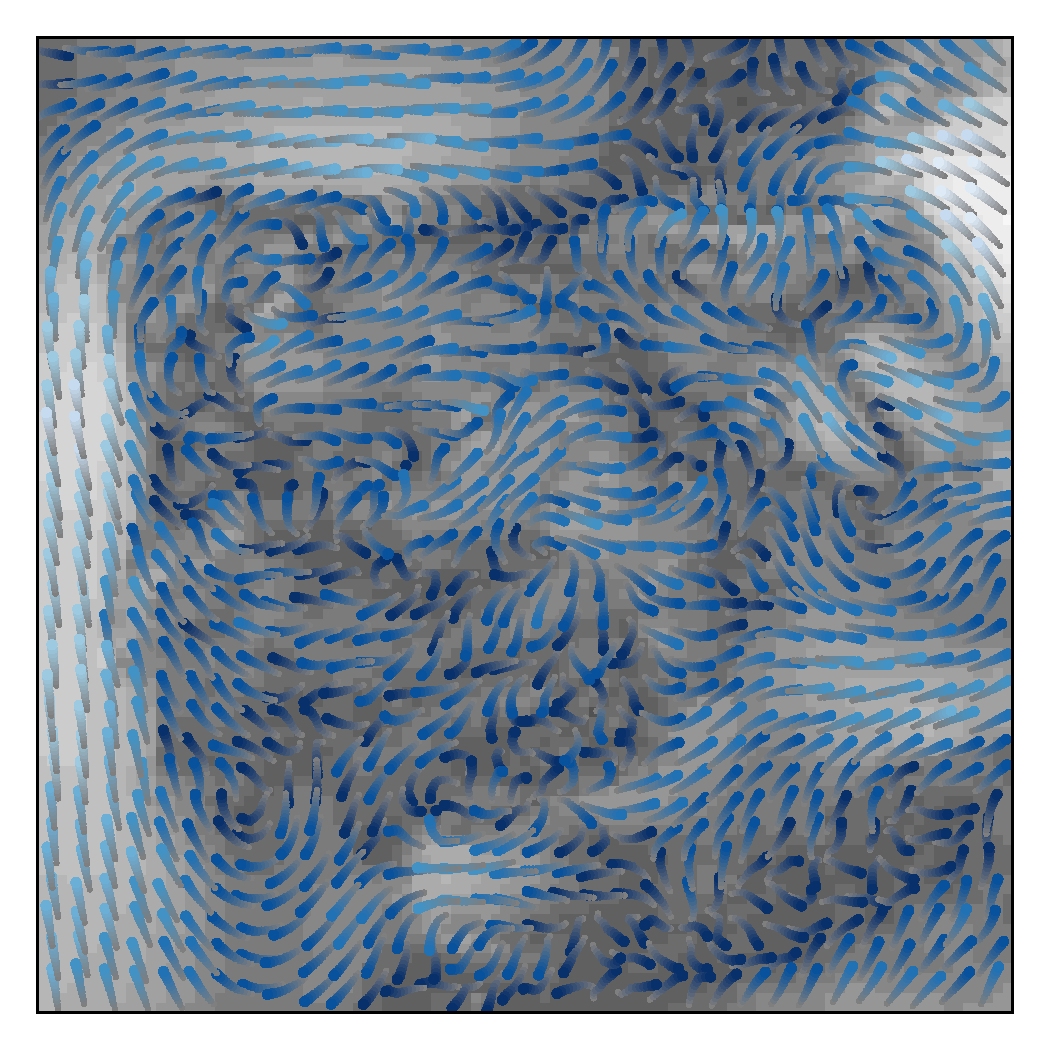
\includegraphics[width=.9\linewidth]{figs/streamplot.pdf}
\caption{\label{fig:streamplot}Streamlines of the wind vector field.}
\end{figure}

The magic of Figure \ref{fig:streamplot} is that it is able to show the
underlying physical structure of the spatial region only displaying
wind speed and direction. It is easy to recognize the Iberian
Peninsula surrounded by strong winds along the eastern and northern
coasts. Another feature easily distinguishable is the Strait of
Gibraltar, a channel that connects the Atlantic Ocean to the
Mediterranean Sea between the south of Spain and the north of
Morocco. Also apparent are the Pyrenees mountains and some of the
river valleys.
